\documentclass[a4paper, 12pt]{report}
\usepackage{geometry}	
\usepackage[utf8]{inputenc}
\usepackage{amsmath}
\usepackage{multicol}
\usepackage{titlesec}
\usepackage{graphicx}
\usepackage{wrapfig}
\usepackage{textcomp}
\usepackage{caption}
\usepackage{subcaption}
\usepackage{comment}
\usepackage{etoolbox}
\usepackage{anyfontsize}
\usepackage{url}
\usepackage{multirow}
\usepackage{array}
\usepackage{tabu}
\usepackage{color}
\usepackage{epigraph}
\usepackage{makebox}
\usepackage{graphicx}
\usepackage{array}
\usepackage{setspace}
\usepackage{natbib}
\usepackage{mathrsfs}
\usepackage{caption}
\usepackage{float}
\usepackage{makecell}
\usepackage[hang, flushmargin]{footmisc}
\usepackage[colorlinks=false]{hyperref}
\usepackage{footnotebackref}
\usepackage{listings}
\lstset{language=python} 

\captionsetup{font={stretch=1.2}}
\usepackage[english]{babel}
\graphicspath{{C:/Users/User/Desktop/images/}}

% BASIC FORMAT SETTINGS
\renewcommand{\arraystretch}{2}
\renewcommand{\bibname}{REFERENCES}
\hypersetup{
    colorlinks,
    citecolor=black,
    filecolor=black,
    %linkcolor=[RGB]{0,204,0},
    linkcolor=black,
    urlcolor=black
}

% \captionsetup[figure]{labelfont=bf, font=footnotesize}

\setlength{\parskip}{1em}
% \setcounter{tocdepth}{4}
% \setcounter{secnumdepth}{4}

%this several lines is for: no number before suction. (This is a bug)
\makeatletter
\patchcmd{\ttlh@hang}{\parindent\z@}{\parindent\z@\leavevmode}{}{}
\patchcmd{\ttlh@hang}{\noindent}{}{}{}
\makeatother


\geometry{
	a4paper,
	% total={210mm,297mm},
 	left=30mm,
 	top=30mm,
  right=30mm,
  bottom=30mm,
}

\newcommand{\mycaption}[1]{\protect \caption{#1}}
%Below is the main content.

%insert a single figure.
%parameters: 
%%  1. path
%%  2. scale
%%  3. caption
\newcommand{\singleFig}[3]{
  \begin{figure}[!htp]
    \centering
    \includegraphics[scale=#2]{#1}
    \caption{#3}
    \label{fig: #1}
  \end{figure}
}

\newcommand{\doubleFig}[6]{
  \begin{figure}[!ht]  
    \begin{center}
    \begin{minipage}{0.45\textwidth}
      \begin{center} 
          \includegraphics[scale=#2]{#1}
      \end{center}
    \end{minipage}
    \begin{minipage}{0.45\textwidth}
      \begin{center} 
          \includegraphics[scale=#4]{#3}
      \end{center}
    \end{minipage}
  \end{center}
  \begin{center}
    \caption[#5]{#6}
    \label{fig: #1-#3} 
    \end{center} 
  \end{figure}
}


\newcommand{\gj}[0]{
  Goldreich-Julian charge density
}

\newcommand{\fgl}[0]{
  \textit{Fermi} LAT four-year Point Source Catalog
}

\newcommand{\question}[1]{
  $<$\textbf{question}$>$#1$<$\textbf{/question}$>$
}

\newcommand{\change}[1]{
  $<$\colorbox{red}{\textbf{change}}$>$#1$<$\colorbox{red}{\textbf{/change}}$>$
}

\newcommand{\add}[1]{
  $<$\colorbox{red}{\textbf{add}}$>$#1$<$\colorbox{red}{\textbf{/add}}$>$
}

\newcommand{\mayAdd}[1]{
  $<$\colorbox{red}{\textbf{mayAdd}}$>$#1$<$\colorbox{red}{\textbf{/mayAdd}}$>$
}


\newcommand{\mayChange}[1]{
  $<$\colorbox{red}{\textbf{mayChange}}$>$#1$<$\colorbox{red}{\textbf{/mayChange}}$>$
}

\newcommand{\myComment}[1]{
  %#1 
  \newline
}

\newcommand{\Notice}[1]{
  $<$\textbf{Notice}$>$#1$<$\textbf{/Notice}$>$
}

\newcommand{\blackhref}[2]{
  \href{#1}{\color{black}{\textit{\small #2}}}
}


\newcommand\aj{AJ}

\newcommand\apj{ApJ}

\newcommand\apjl{ApJL}

\newcommand\apjs{ApJS}

\newcommand\araa{ARA\& A}

\newcommand\mnras{MNRAS}

\newcommand\nat{Nature}

\newcommand\pasp{PASP}

\newcommand\procspie{Proc. SPIE}



\title{\textbf{Identify Exoplanet Candidates with Deep Learning Models} \\ \vspace{1cm}
  {\large Department of Physics, The University of Hong Kong, Pokfulam Road, Hong Kong}}

\date{}
\author{Wang Wenchao  \\3030053350}
\setlength{\columnsep}{1cm}


\begin{document}

\begin{titlepage}
  \begin{center}
  \vspace*{3cm}
  % Gamma-ray Spectral Analysis of Three Energetic Millisecond Pulsars
  \Large \textbf{IDENTIFY EXOPLANET CANDIDATES \\[0.5cm]WITH DEEP LEARNING MODELS\\[0.5cm]}
  \small
    A THESIS \\[0.5cm] 
    SUBMITTED TO THE DEPARTMENT OF PHYSICS \\[0.5cm]
    OF THE UNIVERSITY OF HONG KONG \\[0.5CM]
    IN PARTIAL FULFILLMENT OF THE REQUIREMENTS \\[0.5cm]
    FOR THE DEGREE OF \\[0.5cm]
    DOCTOR OF PHILOSOPHY \\[4.2cm]

    By \\[0.5cm]
    \large Wenchao Wang \\[0.5cm]
    August 2021
    \newpage 
    \centering 
    Abstract of thesis entitled \\[1.2cm]
    \Large \textbf{IDENTIFY EXOPLANET CANDIDATES \\[0.5cm]WITH DEEP LEARNING MODELS\\[0.5cm]}
    \normalsize Submitted by \\ [0.5cm]
    \Large \textbf{Wenchao Wang} \\[1cm]
    \normalsize for the degree of Doctor of Philosophy \\[0.5cm]
    at the University of Hong Kong \\[0.5cm]
    in August 2021 \\[1.9cm]
  \end{center}

    % abstract
    \doublespacing
    \noindent The work is about identifying planet candidates using deep learning models.
Finding these objects manually is a very labor intensive task.
For example, \textit{The Large
    Synoptic Survey Telescope (LSST)} is expected to generate about
$200,000$ images per year, which is equivalent of more than
$10^{6}$ GB of data. Therefore using reliable algorithms to
manage the data is necessary. Deep learning can be helpful
because it suits well for very large input data. In general,
having more data only makes deep learning models perform better.

\vspace{\baselineskip}

\noindent We use \textit{Kepler Space Telescope} and
\textit{Transiting Exoplanet Survey Satellite} (\textit{TESS})
to detect planet candidates by using a convolutional neural
network model. We apply the Q1-Q17 (DR24) table as our training
and test sets. The model takes
two phase-folded light curves and some parameters of each transit-like signal
and then outputs whether the signal represents a planet candidate (PC), 
a non-transiting phenomena (NTP) or a false positive (FP).
In the current model, we feed 17 features into a dense neural network
model, such as transit durations and depth of signals.
At this stage, the models achieve AUROC and accuracy
of about $97.7\%$, $95.9\%$ respectively for the test set.
The accuracy for the training set can be over $99\%$, which means that
the model can easily overfit the data. The most straightforward way to the
problem is to use more data to train the model.
Therefore, we plan to train it with more simulated data later in order to
increase the AUROC and accuracy of predictions.
    
\end{titlepage}

\bibpunct{(}{)}{;}{a}{}{,}
\bibliographystyle{apj}

\linespread{1.25}
\maketitle

\pagenumbering{roman}

% DECLERATION
\cleardoublepage

\chapter*{Declaration}
  \doublespacing 
  I hereby declare that this whole dissertation report is my own work, except the parts with due
  acknowledgment, and that it has not been previously included in a thesis, dissertation or
  report submitted to this University or to any other institution for a degree, diploma or other
  qualifications. \\ \vspace{3cm}

  \hspace{7cm} Signature: \rule{3cm}{0.4pt} 

  \hspace*{7.5cm} Name:  Wenchao Wang 

  \hspace*{7.6cm} Date:  August 2018 

\addcontentsline{toc}{chapter}{Declaration}


% ACKNOWLEDGMENTS
\cleardoublepage
\chapter*{Acknowledgments}
  \doublespacing
  Lots of people give me much precious help. First of all, I really appreciate my 
  supervisor Dr. Stephen Chi Yung Ng for his great support, patience and kindness. Prof. Takata 
  also provides me much help in term of pulsars' emission mechanisms and numerical simulations and 
  is really charming. In addition, I thank Ms. Ruby Cho Wing Ng for her invaluable guidance and 
  advice. They give me not only knowledge and techniques but also encouragements. Therefore, I 
  would like to express my most sincere thanks to them. 
\addcontentsline{toc}{chapter}{Acknowledgments}

% ABSTRACT
\cleardoublepage
\chapter*{Abstract}
  \doublespacing
  \noindent The work is about identifying planet candidates using deep learning models.
  Finding these objects manually is a very labor intensive task.
  For example, \textit{The Large
      Synoptic Survey Telescope (LSST)} is expected to generate about
  $200,000$ images per year, which is equivalent of more than
  $10^{6}$ GB of data. Therefore using reliable algorithms to
  manage the data is necessary. Deep learning can be helpful
  because it suits well for very large input data. In general,
  having more data only makes deep learning models perform better.
  
  \vspace{\baselineskip}
  
  \noindent We use \textit{Kepler Space Telescope} and
  \textit{Transiting Exoplanet Survey Satellite} (\textit{TESS})
  to detect planet candidates by using a convolutional neural
  network model. We apply the Q1-Q17 (DR24) table as our training
  and test sets. The model takes
  two phase-folded light curves and some parameters of each transit-like signal
  and then outputs whether the signal represents a planet candidate (PC), 
  a non-transiting phenomena (NTP) or a false positive (FP).
  In the current model, we feed 17 features into a dense neural network
  model, such as transit durations and depth of signals.
  At this stage, the models achieve AUROC and accuracy
  of about $97.7\%$, $95.9\%$ respectively for the test set.
  The accuracy for the training set can be over $99\%$, which means that
  the model can easily overfit the data. The most straightforward way to the
  problem is to use more data to train the model.
  Therefore, we plan to train it with more simulated data later in order to
  increase the AUROC and accuracy of predictions.
			
\addcontentsline{toc}{chapter}{Abstract}

\tableofcontents

\cleardoublepage
\phantomsection
\addcontentsline{toc}{chapter}{\listfigurename}
\listoffigures
% \newpage

\cleardoublepage
\phantomsection
\addcontentsline{toc}{chapter}{\listtablename}
% \newpage

\pagenumbering{arabic}
 
\cleardoublepage
\newpage
\listoftables

% INTRODUCTION

\chapter{Introduction}
  \section{Transit Photometry}
    A planet is too faint to be found directly by telescopes, so people study it 
    by observing its 
    host star. Since planets orbit around their host stars, they have some periodical effects 
    on the stars such as gravitational pull and light blocking. When a exoplanet pass in front 
    of its host star, it blocks a very small fraction of the star. By measuring the drops of  
    the starlight, basic stats of the planet can be obtained such as period and size. 

    Because planets are in general very tiny compared to host stars, the drops of the 
    starlight are very small. Therefore, some statistic methods are used to identify 
    transits. The confirmed transits that passed statistic tests are called TCE 
    (Threshold-Crossing Events).
    In \textit{Kepler} DR24 data products (the data used in this thesis), 
    the mean and median of TCE are 
    about $12516$ ppm and $125$ ppm respectively (ppm stands for Parts Per Million). The 
    distribution of TCE depths is shown in the following figures.

    \begin{figure}[!htp]
      \centering
      \includegraphics[scale=0.7]{tce_depth_hist.png}
      \caption[The distribution of TCE depths of \textit{Kepler} DR24 data.]
      {The distribution of TCE depths of \textit{Kepler} DR24 data. There are 20367 TCE
      in the data and only 1831 are larger than 10000 ppm (less than 10\%). 
      The histogram shows that most of TCE depths are smaller than 500 ppm.}
    \label{fig: tce_hist_and_pie} 
    \end{figure}

  
  \section{\textit{Kepler Space Telescope}}
    \textit{Kepler Space Telescope} is a space telescope for finding
    Earth-like terrestrial exoplanets. It was launched on March 7th, 2009 and 
    was retired in late 2018. During its service, \textit{Kepler Space Telescope} observes
    more than 500 thousand stars and finds about 2600 exoplanets.
    
    The \textit{Kepler} pipeline is a set of programming tools which can generate
    calibrated light curves which can then be fed into the
    algorithms to discriminate between planet candidates (PC) and other types of light curves.
    Threshold Crossing Events (TCE) are generated
    after Transiting Planet Search (TPS) which is part of 
    the \textit{Kepler} pipeline. And then we can identify planet candidates
    by analyzing the generated TCE. 

    \textit{Kepler} team developed a tool called \textit{Kepler Robovetter} 
    \footnote{https://github.com/nasa/kepler-robovetter}
    to identify PCs and false positives and it achieves a high accuracy (over 97\%).
    It is a traditional algorithm which is purely written in C++ and 
    is very fast. However, it is difficult to understand
    and one can view its source code on the github. Therefore, try different method like 
    machine learning may be a feasible choice.
  
  \section{Machine Learning}
      Machine learning is a subset of artificial intelligence and has been successfully used 
      in many areas for a variety of tasks such as self-driving cars and optical character
      recognition (ORC) which can extract words and their meanings from images. Machine 
      learning methods can even generate art works such as pictures which are nearly 
      indistinguishable from art works created by artists. Therefore, it is natural to think 
      that machine learning methods can also be applied to astronomy. 

      Machine learning can be classified differently based on different criteria. For example,
      if we predict a product's price which is a concrete value, we are doing a regression task. 
      Otherwise, if we need to classify pictures as dogs or cats, then it is a classification 
      task. Meanwhile, an algorithm is called supervised learning if we train the machine 
      learning model by giving corresponding labels. Otherwise, it is a 
      non-supervised learning algorithm. In this thesis, we input the TCE with 
      corresponding category labels generated by 
      \textit{Kepler} pipeline and output a number 0 or 1 to indicate PC or non-PC. Thus,
      we use a supervised learning method to do a classification task.

      There are a large quantity of machine learning algorithms for classification tasks
      such as logistic regression, decision trees and support vector machines. However, 
      in this thesis, besides trying these machine learning methods, we 
      focus more on deep learning methods, especially convolution neural networks (CNN).


  

% DATA PREPARATION
\chapter{Data Preparation}
  As previously mentioned, we use \textit{Kepler} DR24 data 
  \footnote{ https://exoplanetarchive.ipac.caltech.edu/docs/Kepler\_TCE\_docs.html}
  with labels to train out model. It is a CSV file while other types are also 
  supported. Note that the data contains training labels generated by autovetter which 
  is basically a
  random forest technique. Random forest is also a supervised machine learning algorithm,
  thus it also needs labels to tell the algorithm which one is PC. The labels fed into 
  random forest algorithm are classified by humans. The reason why use deep learning method 
  to redo the classification task is because deep learning performs very well when trained 
  with large amount of data. Therefore, we try to use the human-made and normal machine 
  learning method generated labels to train a deep learning model in order to get better 
  accuracy.

  The labels contain four unique values: 
  PC (Planet Candidates) , AFP (Astronomical False Positive), NTP 
  (Non-transiting Phenomenon) and UNK (Unknown). There are 27 columns in the data including 
  the label column named "av\_training\_set". Each other column represents a property of one 
  TCE and some of the columns are more important for our classification task, such as 
  "tce\_period", "tce\_duration", "tce\_prad", "tce\_depth", etc. Meanings of the some 
  column names are listed in the following table.
  \footnote{https://exoplanetarchive.ipac.caltech.edu/docs/API\_tce\_columns.html}

  \begin{table}[!htp]
    \centering
    \scalebox{0.8}{
    \begin{tabular}{|c|c|} 
      \hline 
      \textbf{Column Name} & \textbf{Definition} \\
      \hline 
      tce\_period & time interval between two consecutive transits in days \\
      \hline 
      tce\_depth & starlight drops in ppm \\
      \hline 
      tce\_prad & the planet radius in Earth Radii \\
      \hline 
    \end{tabular}}
    \centering
    \caption[Descriptions of column names.]{Descriptions of column names. The listed 
      properties are more important for identifying PC.}
    \label{table: difinitions_of_column_names}
  \end{table}
  
  The CSV table needs to be preprocessed. First of all, we need to drop all data labeled with 
  'UNK'. Then since deep learning algorithms only deal with numerical labels, we need to 
  label PC and non-PC as 1 and 0 respectively. Non-PC includes both AFP and NTP because we do 
  binary classification to find out planet candidates. After processing the basic properties 
  for each TCE, we also need to download their light curves.

  \section{Download Light Curves}
    Light curves are downloaded based on the column name "kepid" in the \textit{Kepler} DR24 
    data table previously discussed. There are about 16 fits files which is composed of four 
    year observation corresponding to a kepid. All the light curves can be found on the 
    website \blackhref{https://archive.stsci.edu/pub/kepler/lightcurves/0020/}
    {https://archive.stsci.edu/pub/kepler/lightcurves/0020/}. A tricky thing is that 
    there are 20367 TCE
    in the table containing more than 330,000 light curve files. Downloading these 
    files can be very time consuming (about 2 weeks by estimation). Therefore, I scrape the 
    webpage in parallel to filter the light curves data and download them. 

    Take kepid 000757137 as an example. The URL of the light curves for this TCE is 
    \blackhref{http://archive.stsci.edu/pub/kepler/lightcurves/0007/000757137}
    {http://archive.stsci.edu/pub/kepler/lightcurves/0007/000757137}. There are 17 light 
    curve files as the following screen shot shown.
    \begin{figure}[!htp]
      \centering
      \includegraphics[scale=0.4]{kepid_light_curves_example.PNG}
      \caption{The screen shot of webpage containing light curves of kepid 000757137}
      \label{fig: kepid_light_curves_example}
    \end{figure}

    We can find the hyper link from the anchor tag and navigate to the URL of the desired 
    data. The code is written in Golang, which is very good at concurrency. All code can be 
    found on \blackhref{https://github.com/grewwc/exoplanet}{github}.
    In short, the basic procedure is 
    \begin{enumerate}
      \item Parse all the hyperlinks from the root URL: \\
        \blackhref{http://archive.stsci.edu/pub/kepler/lightcurves}
        {http://archive.stsci.edu/pub/kepler/lightcurves}. Join the current URL with 
        the parsed hyperlinks to generate new URLs. 
      \item Launch new goroutine to search from the newly generated URLs.
      \item Get the hyper links from the child URLs. If the hyper links are fits files, 
        then download them to a local directory in parallel. 
        Otherwise, as the procedure 1, get new 
        URLs and launch new goroutine to do the search recursively.
    \end{enumerate}

    Another problem is if I search from too many URL simultaneously, my IP will be blocked
    temporarily. Therefore, I need to control the total amount of processes. After some 
    attempts, I find that 200 processes are good enough and all light curves can be 
    downloaded within 3 hours. The point is data are usually very large and complex 
    in the field of astronomy, thus dealing with data efficiently is important.

    
  \section{Light Curves Pre-processing}
    As previously discussed, the depths of TCE are in general very small and the median 
    value is around 125 ppm. The following figure is the four-year observation data. 
    Thus we need to fold the light curves and bin them in order to magnify the effect.
    Moreover, we can see some data points in the top right side of the figure. We also 
    need to remove the outliers to improve out model's prediction accuracy.
    
    \begin{figure}[!htp]
      \centering
      \includegraphics[scale=0.6]{11442793_time_flux.png}
      \caption[Plot of normalized flux to time of kepid 11442793.]
        {Plot of normalized flux to time of kepid 11442793. The flux is normalized by 
        dividing the original flux by their median value.}
      \label{fig: 11442793_time_flux}
    \end{figure}

    In addition, there is long-term trend which is clearly not a transit signal
    in the light curves for some kepids. For example, we can see a clear periodical 
    fluctuation in the light curve for kepid 1164109 as the following figure shown.
    The fluctuation has bad effects for the deep learning model, thus even though we don't 
    have to deal with the long-term trend, removing the trend may increase the model's 
    performance.

    \begin{figure}[!htp]
      \centering
      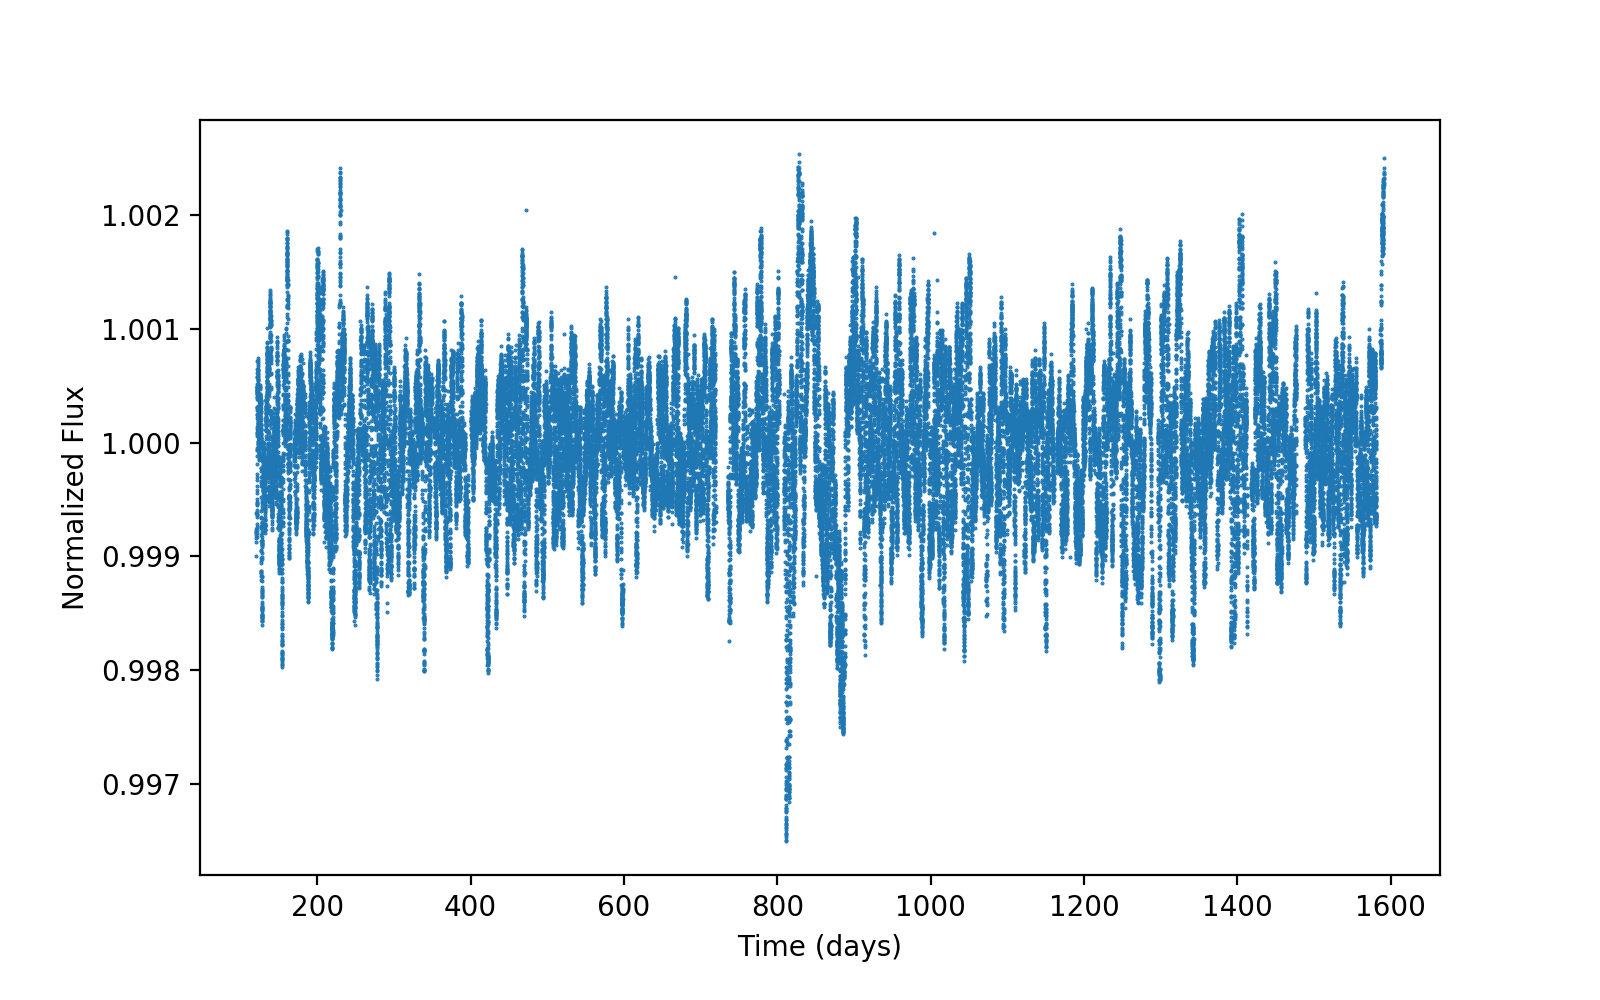
\includegraphics[scale=0.5]{1164109_time_flux.png}
      \caption[Plot of normalized flux to time of kepid 1164109.]
        {Plot of normalized flux to time of kepid 1164109.}
      \label{fig: 1164109_time_flux}
    \end{figure}

    Finally, since there may be more than one planet associated with a kepid, we remove 
    signals of other planets in the same system to avoid interference. The complete 
    progress of light curves preprocessing is described as follows.

    \subsection{Remove Multiple Signals in the Same Stellar System}
      The following table shows some useful parameters of TCE for kepid 1162345. 
      When preprocessing kepid 1162345, we fetch all the TCE --- there are 3 TCE in the stellar 
      system. Then we process the TCE one by one, with other two TCE removed. The remove logic is simple:
      mask out the data points within the range [center-duration, center+duration] and return the new 
      flux and time pairs. 

      \begin{table}[!htp]
        \centering
        \scalebox{0.8}{
        \begin{tabular}{|c|c|c|c|} 
          \hline 
          \textbf{tce\_plnt\_number} & \textbf{tce\_period (day)} & \textbf{tce\_duration (hr)} & \textbf{tce\_depth (ppm)} \\
          \hline 
          2	& 0.831850 & 2.392 & 2.636\\
          \hline 
          3	& 0.831833 & 2.181 & 27.100\\
          \hline 
          1	& 0.831777 & 2.349 & 24.270	\\ 
          \hline 
        \end{tabular}}
        \centering
        \caption[Parameters of three TCE for kepid 1162345.]
          {Parameters of three TCE for kepid 1162345. When processing the TCE for planet 2, we remove the signals for 
          planet 1 and 3.}
        \label{table: params_1162345}
      \end{table}
    
    \subsection{Remove Outliers and Long-term Trend}
      Before doing further processing to the light curves, we need to remove the outliers 
      first to increase our model's performance. We just use a simple sigma clip to do the 
      job. The method firstly derive the median and standard deviation value
      of the flux ($m, \sigma$). Then any points not within the range of $m \pm n\sigma$ 
      are removed, where n is a parameter with default value of 3.

      Then we should remove the long-term trend in the light curves. 
      In this thesis, we use a python package called lightkurve 
      \footnote{https://docs.lightkurve.org/} which internally uses 
      Savizky-Golay filter to remove the low-frequency trend. The lightkurve package 
      contains an python object called LightKurve which has a "flatten" method. After 
      some experiments, we change some default parameter values as the following table shown:

      \begin{table}[!htp]
        \centering
        \scalebox{0.8}{
        \begin{tabular}{|c|c|c|c|c|} 
          \hline 
           & \textbf{window\_length} & \textbf{polyorder} & \textbf{break\_tolerance} & \textbf{sigma} \\
          \hline 
          \textbf{values} & 201 & 2 & 40 & 3 \\
          \hline
        \end{tabular}}
        \centering
        \caption[Parameter values chosen in the LightKurve flatten method.]
          {Parameter values chosen in the LightKurve flatten method. The detailed 
          descriptions of these parameters can be found on the lightkurve official 
          website.}
        \label{table: params_1162345}
      \end{table}

      Take kepid 1164109 for example, the following figures are original normalized flux 
      and flattened flux. After removing the long-term trend from the original normalized 
      light curve, the transit signal becomes more clear. 

      \begin{figure}[!ht]  
        \begin{center}
        \begin{minipage}{0.45\textwidth}
          \begin{center} 
              \includegraphics[scale=0.35]{original__1164109.png}
          \end{center}
        \end{minipage}
        \begin{minipage}{0.45\textwidth}
          \begin{center} 
              \includegraphics[scale=0.35]{flattened_1164109.png}
          \end{center}
        \end{minipage}
      \end{center}
      \begin{center}
        \caption[Comparison between original light curve and flattened light curve.]
          {Comparison between original light curve and flattened light curve. The right 
          panel is the normalized light curve of kepid 1164109 after flattening. }
        \label{fig: 1164109_comparison}
        \end{center}
      \end{figure}

    \subsection{Fold and Bin Light Curves}
      First of all, we fold the flattened light curves to increase the data points within 
      the range of the transit signals. Then we move the transit signal in the center 
      of the folded light curve. This may increase the performance of the deep learning model 
      since the data is more "clean". Then we need to bin the folded light curves for the 
      following benefits. 
      \begin{itemize}
        \item There are too many data points in the folded light curves 
          (around 65000 for each folded light curve). 
          As we know, the number of "useful" data points which are within the range of a 
          TCE's duration is very small. Therefore, most of the 65000 data points are 
          nearly "useless" and will waste a lot of computing power. 
        \item Binning can make the light curves a bit more smoother and reduce variants.
          Since a complex machine learning model tend to fit the variants and causes
          over-fitting, which is very bad for the model generalization. Thus, the performance
          of the over-fitted model tend to perform bad on the unseen data.
      \end{itemize}

      There are some python packages such as lightkurve to do the binning operation, however, 
      we can only choose the bin width ($w$) or number of bins. And the distance between 
      each bin ($d$) is equal to the bin width ($d=w$). But these two values can be different:
      if $d<w$, the binned light curves can be more smooth and may can improve the model's 
      performance. Therefore, we need to write our own bin method. Even though the logic 
      of binning method is simple, it is a little bit tricky to implement. For example, if the bin width is so small that there is no data points in this range, what value 
      should we choose to 
      represent this bin? In this thesis, we choose the median value if the bin has no 
      data points. Another question is should we choose the same 
      bin width and distance for all the light curves? After some experiments, 
      we don't find a 
      good criteria to tune the binning parameters for each light curve. Therefore, we use 
      the same parameter configuration for all the light curves. Finally, the performance for 
      this method is very important because we need to do 
      many training experiments, thus we have to generate preprocessed light curves for all 
      the TCE multiple times. 

      The binning parameters also have a huge influence on the performance of the model. 
      We use 2048 bins and bin width $w=(time\_max-time\_min)/num\_bins*1.5$.


% setting for reference 
\bibliography{bibfile}

\end{document}





